
%----------------------------------------------------------------------------------------
%	10./ Sensitivity
%----------------------------------------------------------------------------------------
%\section{Sensitivity}
%\label{se:sensitivity}
%
%----------------------------------------------------------------------------------------
%	10./ Sensitivity
%----------------------------------------------------------------------------------------
%\section{Sensitivity}
%\label{se:sensitivity}
%
%----------------------------------------------------------------------------------------
%	10./ Sensitivity
%----------------------------------------------------------------------------------------
%\section{Sensitivity}
%\label{se:sensitivity}
%
%----------------------------------------------------------------------------------------
%	10./ Sensitivity
%----------------------------------------------------------------------------------------
%\section{Sensitivity}
%\label{se:sensitivity}
%\input{Sensitivity.tex}

In this section, we derive the on-sky sensitivity of the instrument
using a large amount of observation scans, including deep integration
on faint sources, to assess our result stability against the observing
conditions. We evaluate the noise equivalent flux
density, NEFD hereafter, that is the flux density
$1\,\sigma$ errors in one second of effective
on-source telescope integration time after the baseline calibration
has been performed, as described in
Sect.~\ref{se:baseline_calibration}. The first step for
the NEFD measurement is thus an accurate evaluation of the on-source
integration time, which is addressed in
Sect.~\ref{se:integration_time}. Then, for robustness test of the NEFD
estimates, we have devised several methods for estimating the NEFD. A
detailed description of our methods, as well as an application to a
faint source blind detection, will be found in
\citet{Ponthieu2019}. In Sect.~\ref{se:nefd_method}, we briefly
present the NEFD estimation methods that have been used and the data
sets that have been selected. Finally, the NEFD estimates and the
results of the robustness tests we performed are reported in
Sect.~\ref{se:nefd_results}.


\subsection{Estimation of the time of integration}
\label{se:integration_time}

Considering an observation scan of a point-like source, from which we
produce a map by projecting the calibrated TOI (see
Sect.~\ref{se:dataproc}) into pixels of size $\Delta r$, we primarily
estimate the time of integration on-source, which is the integration
time in a beam $t_{\rm{beam}}$, using
%
\begin{equation}
  t_{\rm{beam}} = \frac{<N_{\rm{hit}}>_{\rm{center}}}{f_{\rm{sam}}}\,
  \eta \frac{g^2}{\Delta_r^2},
  \label{eq:integration_time}
\end{equation}
%
where $N_{\rm{hit}}$ is the so-called hit map, that is the map of the
TOI sample count per map pixels, and $<N_{\rm{hit}}>_{\rm{center}}$
is the average of the hit map over the pixels within a FWHM radius
from the center of the map. The ratio of this quantity to the sampling
frequency $f_{\rm{sam}}$ thus corresponds to the total time of integration
spend in a map pixel of the center of the map. As all the KIDs of an
array produce a data sample at the same time, we need to correct the
total time of integration from the fraction of the KID that
contributes to a map pixel at the same time. For this purpose, first
we estimate the number of KID per map pixel as the ratio of $g^2$ to
$\Delta_r^2$, where $g$ is the distance between neighbour KIDs (see
Sect.~\ref{se:grid_distortion}). Then, we multiply
this quantity by the fraction of valid KID $\eta$ that actually
contribute to the map (see Sect.~\ref{se:avg_kidpar}). 

For cross-checks, we compare the $t_{\rm{beam}}$ estimates using an
alternative approach for evaluating the on-source integration
time based on geometrical considerations. Namely, we calculate the
fraction of the scanning time during which the point source in within
an effective FOV radius, which is defined as the FOV covered by the
valid KIDs. We find the two methods to give comparable integration
time estimates to better than $5\%$. We conclude the $t_{\rm{beam}}$
estimates to be reliable and use it for the NEFD derivation.  


\subsection{NEFD estimation methods and source selection}
\label{se:nefd_method}

We have devised three complementary methods for the
NEFD estimation, which come in two different flavours. First, we
use deep integrations on faint sources, and second we resort to 
joint analysis of multiple scans without combining them. An
extensive discussion of these methods will be given in
\citet{Ponthieu2019}. In this section, we briefly describe one method
for each of the two approaches: \\

\noindent \emph{Deep integration method:} The error on the flux
density of a point source for an integration time $t$ is
$\sigma_\phi(t) = NEFD/\sqrt{t}$. Using long-time integration
observation on a source, we can study the decrease of $\sigma_\phi$
with increasing $t$, and therefore estimate the NEFD if the
different elevation and opacity conditions of observations are
correctly accounted for.
We produce a series of maps using an inverse-variance co-addition of
more and more observation scans, and perform a photometric analysis on
each map according to Sect.~\ref{se:photometry}. Since all the scans
are not acquired in the exact same conditions of atmospheric opacity
and observing elevation, they do not contribute with the same weight
to the co-addition. To derive the top-of-atmosphere NEFD, quoted
NEFD$_0$, we account for the scan-to-scan weighting variations by fitting
the $1\sigma$ flux errors with
\begin{equation}
  \sigma(n) = \frac{NEFD_0}{\sqrt{\sum_{i=1}^{n}t_i e^{-2\tau_i/\sin\delta_i}}},
  \label{eq:sigma_tau_w8}
\end{equation}
where $t_i$, $\tau_i$ and $\delta_i$ are the integration time, the
zenith opacity and the observing elevation of the $i$-th scan of the
$n$-scan co-addition. The quantity $\sum_{i=1}^{n}t_i
e^{-2\tau_i/\sin\delta_i}$ thus consists in an
estimate of the effective integration time for the series of scans
that enter the $n$-scan co-addition. \\

\noindent \emph{Scatter method:} Performing photometry on each
individual scan, we can estimate the sensitivity on the central flux
and measure the time of integration using
Eq.~\ref{eq:integration_time}, hence derive the NEFD for this
scan. After correction of the attenuation of the atmosphere, the joint
analysis of a series of scans provides us with an estimate of the
top-of-atmosphere NEFD. \\

The selection of the source target for the NEFD derivation is
primarily based on the flux density. Indeed, noise
characterization may be biased by residuals of a strong source and the
instrument far side lobes. For the scatter method, we therefore
restrict the analysis to sources with a flux below 1\,Jy. For the deep
integration method, we further need to select a single source whose
visibility allows for long integration time. During the N2R9 campaign,
we selected \hls\, which is a
moderately faint source \citep{hls_combes}, expected to be
74.5\,mJy at 1mm and 15.7\,mJy at 2mm (M.~Bethermin, private
communication). It has been observed for about 9\,h in total over
three nights using 8x5~arcmin$^2$ OTF scans of various orientations. 

\begin{figure*}[!thbp]
  \begin{center}
    \includegraphics[trim={0.5cm, 0.5cm, 1.5cm, 1.8cm}, clip, angle=0, width=0.495\textwidth]{Figures/hls_nefd_vst.eps}
    \includegraphics[trim={0.5cm, 0, 0.2cm, 0.5cm}, clip, angle=0, width=0.485\textwidth]{Figures/hls_NEFD_vs_TauElev_all.eps}
    \caption{Comparison of NEFD estimates using two methods on
      observation of \hls. \emph{Left panel:} Evolution of the 1\,$\sigma$ flux density uncertainties as a function of the integration time; \emph{Right panel:} NEFD as a function of the measured line-of-sight opacity. The solid black line is the theoretical fit of $\rm{NEFD} = \rm{NEFD}_0$ $e^{(\tau/\sin\delta)}$ and gives the NEFD when extrapolated to $\tau/\sin\delta = 0$.}
    \label{fig:nefd_twomethods}
  \end{center}
\end{figure*}

\subsection{NEFD estimation and robustness tests}
\label{se:nefd_results}

%  comparison entre methods
First we test the stability of the NEFD estimates using the two
methods on a same data set. In Fig.~\ref{fig:nefd_twomethods}, we
present an application of the deep integration method (left panel) and
the scatter method (right panel) on
%the NEFD estimates for Array 1, 3, the combination of A1$\&$A3
%and Array 2 using
the series of \hls\ observation scans.

The left panel of Fig.~\ref{fig:nefd_twomethods} shows the flux density
uncertainties as a function of the integration time. This plot has
been obtained as discussed in Sect.~\ref{se:nefd_method}. The small
variations of the slope of the $1\sigma$ flux errors, which are
visible on the plot, correspond to variations of line-of-sight opacity
during the integration. These variations are taken into account for
evaluating the top-of-atmosphere NEFD using
Eq.~\ref{eq:sigma_tau_w8}. The NEFD estimates for Array 1, 3, the
combination of A1$\&$A3 and Array 2 using the deep  
integration method are given in the first row of
Table~\ref{tab:nefd_summary}.
 
\begin{table}[!htbp]
  \centering
  \caption[]{Stability of the NEFD estimates. Top-of-atmosphere NEFD
    in mJy.s$^{1/2}$ for the two methods described in the text and
    obtained on \hls\ and all sub-Jy sources of runs N2R9,
  N2R12, N2R14. The results given in the last row are based on more
  than a thousand scans, which distribute as 202, 481 and 430 scans of
  N2R9, N2R12 and N2R14 respectively.}
  \label{tab:nefd_summary}
  \begin{tabular}{llrrrr}
    \hline\hline
    \noalign{\smallskip}
    Data set   & Method   & A1      &   A3    &   A1\&A3 &    A2 \\
    \noalign{\smallskip}
    \hline
    \noalign{\smallskip}
    \hls &     $t^{-1/2}$  &  46.6  &    38.4  &    30.4  &   8.5  \\
    %   G2   &    $t^{-1/2}$  &  44.0  &    34.7  &    29.6  &  7.8  \\
         &     Scatter    &  45.7  &    36.3  &    28.5  &   8.2  \\
    \hline
    \noalign{\smallskip}
    N2R9     & Scatter    & 47.0 &  36.9  & 28.8  & 8.4 \\
    N2R12    &            & 47.3 &  36.4  & 30.2  & 8.5 \\
    N2R14    &            & 47.3 &  39.8  & 30.9  & 9.3 \\
    Combined &            & 47.2 &  37.9  & 30.1  & 8.8 \\
    \hline
  \end{tabular}
\end{table}

In addition, we verify that the noise integrates down as expected with
respect to the integration time. Black lines in the left panel of
Fig.~\ref{fig:nefd_twomethods} show the $1\sigma$ error fit with the
inverse of the square root of the integration time. The noise
integration is well consistent with $t^{-1/2}$.

The right panel of Fig.~\ref{fig:nefd_twomethods} show the NEFD
estimates for  Array 1, 3, the combination of A1$\&$A3 and Array 2
using the scatter method, as discussed in Sect.~\ref{se:nefd_method},
as a function of the line-of-sight opacities, $\tau/sin(\delta)$,
where $\tau$ is the zenith opacity and $\delta$ the observing
elevation. The solid lines show the best fit of the model for a
background-dominated sensitivity,
defined as NEFD = NEFD$_0$ exp${[\tau/sin(\delta)]}$. The best-fitting
NEFD$_0$ amplitude give us estimates of the
top-of-atmosphere NEFD, which are gathered in
Table~\ref{tab:nefd_summary}.

We observe systematically higher NEFD for A1 compared to
A3, which is a mainly due to the dichroic-induced 'shadow effect' that
also impacts the flat fields, as discussed in
Sect.~\ref{se:flat_field}. Furthermore, the NEFDs are well consistent
with being background dominated for each array and each observing
wavelength. 


%  comparison entre datasets
As a second robustness test, we check the stability of the NEFD for
three observation
campaigns. Figure~\ref{fig:nefdvsbackground_below_1Jy} shows the
measured NEFD using the scatter method for runs N2R9, N2R12 and
N2R14. 

\begin{figure*}[!thbp]
\begin{center}
%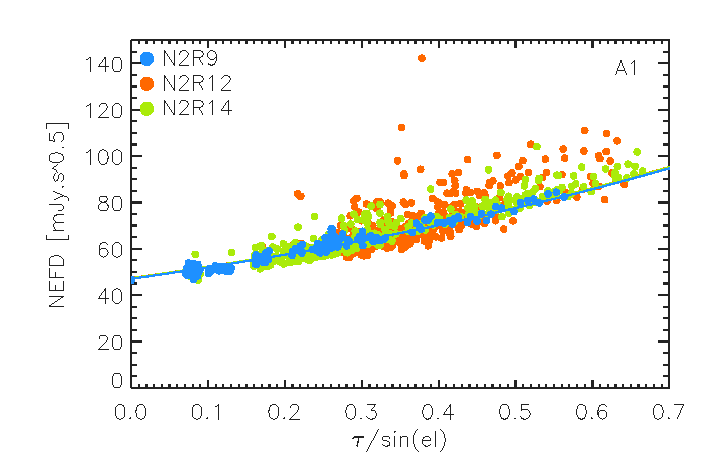
\includegraphics[clip=true,width=0.47\textwidth]{Figures/plot_nefd_vs_obstau_corrected_skydip_vfinal_a1.pdf}
%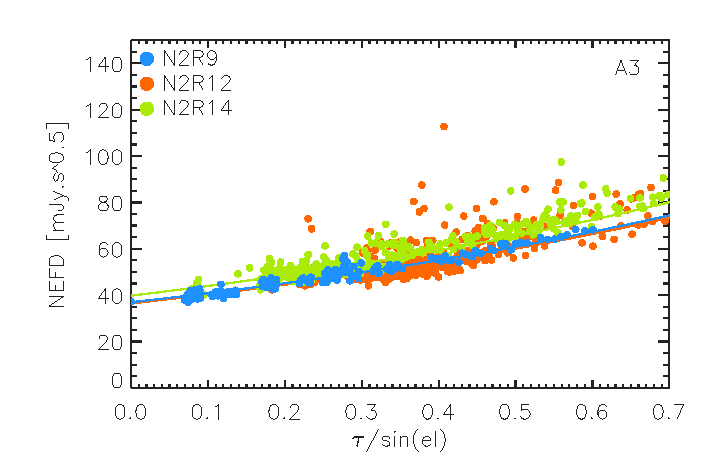
\includegraphics[clip=true,width=0.47\textwidth]{Figures/plot_nefd_vs_obstau_corrected_skydip_vfinal_a3.pdf}
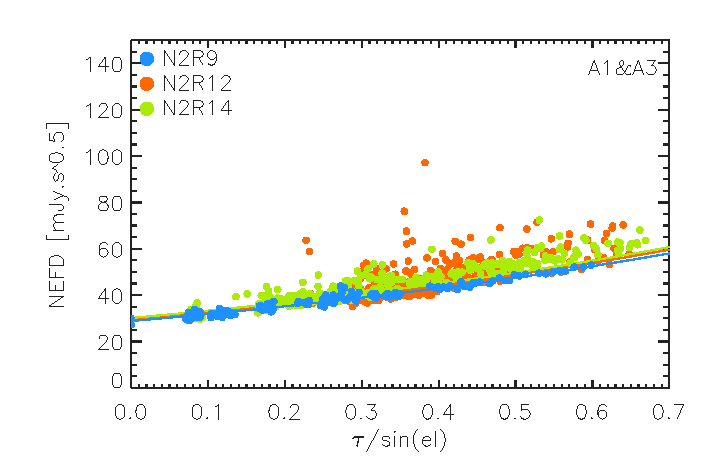
\includegraphics[clip=true,width=0.47\textwidth]{Figures/plot_nefd_vs_obstau_corrected_skydip_vfinal_1mm.pdf}
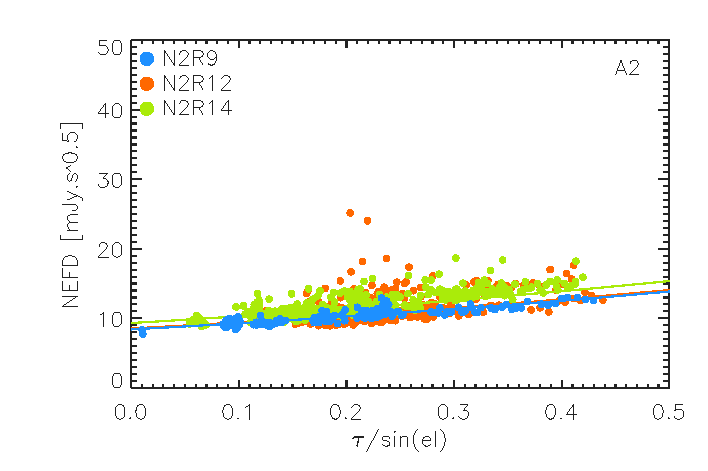
\includegraphics[clip=true,width=0.47\textwidth]{Figures/plot_nefd_vs_obstau_corrected_skydip_vfinal_a2.pdf}
\caption{Comparison of the NEFD estimates for three observation
  campaigns. The measured NEFD using the scatter method is plotted as a function of
  line-of-sight opacity ($\tau/sin(\delta)$) for the $1~\rm{mm}$ (left) and $2~\rm{mm}$ (right)
  channels. Data points are NEFD estimates in mJy.s$^{1/2}$ for N2R9 (blue), N2R12 (orange)
  and N2R14 (chartreuse). We also show in the plots the expected NEFD evolution
  with the line-of-sight opacity as solid curves using the median
  zenith opacity derived from all the scans acquired during a campaign.}
\label{fig:nefdvsbackground_below_1Jy}
\end{center}
\end{figure*}

Combining the data set of N2R9, N2R12 and N2R14 campaigns,
more than one thousand observations scans of sub-Jy sources meet the
baseline selection criteria (see Sect.~\ref{se:data_selection}),
providing us with robust NEFD estimates that are representative of
average NIKA2 performance, which are gathered in
Tab.~\ref{tab:nefd_astro}.
The top-of-atmosphere NEFD and RMS uncertainties are evaluated as the median and
the scatter of the individual NEFD corrected with
$\exp[\tau/sin(\delta)]$. These values are then extrapolated at the
reference IRAM observing conditions, which consists of $2~\rm{mm}$
of precipitable water vapor (pwv) in the atmosphere and $60$ degrees
elevation.


\subsubsection{Mapping speed}

To further estimate the mapping capabilities, we also evaluate the
mapping speed $M_{\rm{s}}$, which is defined as the sky area that is covered in one
hour of observation to a noise level of $1\,\rm{mJy}$, using
\begin{equation}
M_{\rm{s}} = \eta \, \frac{\pi}{4} d_{\rm{FoV}}^2 \, \frac{\Delta_t}{\rm{NEFD}^2},
\end{equation}
where $d_{\rm{FoV}} = 6.5'$ is the FoV diameter, $\eta$ the
fraction of valid KIDs, as given in Tab.~\ref{tab:number_of_kids} in
Sect.~\ref{se:fov_geometry} and $\Delta_t$ a time period of one hour.
The mapping speed that is extrapolated at zero opacity, and the astronomer
mapping speed that is extrapolated at the reference IRAM observing conditions are
given in Tab.~\ref{tab:nefd_astro}.   
%eta  = [0.84, 0.84, 0.84, 0.90]
%nefd0 = [47.2, 37.9, 30.1, 8.8]
%ms0   = !dpi/4.0d0*6.5d0^2*eta/nefd0^2*60.0d0^2 ;; arcmin^2/h/mJy^2
%print, ms0
%nefda = [56.6, 45.6, 36.1, 9.8]
%msa   = !dpi/4.0d0*6.5d0^2*eta/nefda^2*60.0d0^2 ;; arcmin^2/h/mJy^2
%print, msa

\begin{table}[!thbp]
  \begin{center}
    \caption[NEFD estimates on all sub-Jy sources]{Median NEFD and rms
      uncertainties in $\rm{mJy}\cdot \rm{s}^{1/2}$, as well as the derived mapping
      speed in $\rm{arcmin}^2\cdot\rm{mJy}^{-2}\cdot\rm{h}^{-1}$, evaluated
      in using the scatter method on all sub-Jy sources of runs N2R9, N2R12
      and N2R14, given at pwv=0 and 90 degrees elevation (first three rows) and extrapolated at the
      reference IRAM observing conditions (last three rows), which are defined
      as $2\,\rm{mm}$ pwv and 60 degrees elevation.}
    \label{tab:nefd_astro}
    \begin{tabular}{lrrrr}
      \hline\hline
      \noalign{\smallskip}
      <1 Jy               & A1      &   A3    &   A1\&A3 &    A2 \\
      \noalign{\smallskip}
      \hline
      \noalign{\smallskip}
      NEFD\small{(0mm, 90deg)}             & 47.2    & 37.9    &    30.1  &    8.8   \\
      RMS NEFD\small{(0mm, 90deg)}         &  3.9    &  3.5    &     2.9  &    1.1   \\
      M$_{\rm{s}}$\small{(0mm, 90deg)}      & 45      &  70     &    111   &   1388   \\
      \hline
      \noalign{\smallskip}
      NEFD\small{(2mm, 60deg)}         & 56.6    & 45.6    &    36.1  &    9.8   \\
      RMS NEFD\small{(2mm, 60deg)}     &  4.7    & 4.2     &     3.5  &    1.2   \\
      M$_{\rm{s}}$\small{(2mm, 60deg)}  &  31    & 48       &    77   &   1119   \\
      \hline
    \end{tabular}
\end{center}
\end{table}


In this section, we derive the on-sky sensitivity of the instrument
using a large amount of observation scans, including deep integration
on faint sources, to assess our result stability against the observing
conditions. We evaluate the noise equivalent flux
density, NEFD hereafter, that is the flux density
$1\,\sigma$ errors in one second of effective
on-source telescope integration time after the baseline calibration
has been performed, as described in
Sect.~\ref{se:baseline_calibration}. The first step for
the NEFD measurement is thus an accurate evaluation of the on-source
integration time, which is addressed in
Sect.~\ref{se:integration_time}. Then, for robustness test of the NEFD
estimates, we have devised several methods for estimating the NEFD. A
detailed description of our methods, as well as an application to a
faint source blind detection, will be found in
\citet{Ponthieu2019}. In Sect.~\ref{se:nefd_method}, we briefly
present the NEFD estimation methods that have been used and the data
sets that have been selected. Finally, the NEFD estimates and the
results of the robustness tests we performed are reported in
Sect.~\ref{se:nefd_results}.


\subsection{Estimation of the time of integration}
\label{se:integration_time}

Considering an observation scan of a point-like source, from which we
produce a map by projecting the calibrated TOI (see
Sect.~\ref{se:dataproc}) into pixels of size $\Delta r$, we primarily
estimate the time of integration on-source, which is the integration
time in a beam $t_{\rm{beam}}$, using
%
\begin{equation}
  t_{\rm{beam}} = \frac{<N_{\rm{hit}}>_{\rm{center}}}{f_{\rm{sam}}}\,
  \eta \frac{g^2}{\Delta_r^2},
  \label{eq:integration_time}
\end{equation}
%
where $N_{\rm{hit}}$ is the so-called hit map, that is the map of the
TOI sample count per map pixels, and $<N_{\rm{hit}}>_{\rm{center}}$
is the average of the hit map over the pixels within a FWHM radius
from the center of the map. The ratio of this quantity to the sampling
frequency $f_{\rm{sam}}$ thus corresponds to the total time of integration
spend in a map pixel of the center of the map. As all the KIDs of an
array produce a data sample at the same time, we need to correct the
total time of integration from the fraction of the KID that
contributes to a map pixel at the same time. For this purpose, first
we estimate the number of KID per map pixel as the ratio of $g^2$ to
$\Delta_r^2$, where $g$ is the distance between neighbour KIDs (see
Sect.~\ref{se:grid_distortion}). Then, we multiply
this quantity by the fraction of valid KID $\eta$ that actually
contribute to the map (see Sect.~\ref{se:avg_kidpar}). 

For cross-checks, we compare the $t_{\rm{beam}}$ estimates using an
alternative approach for evaluating the on-source integration
time based on geometrical considerations. Namely, we calculate the
fraction of the scanning time during which the point source in within
an effective FOV radius, which is defined as the FOV covered by the
valid KIDs. We find the two methods to give comparable integration
time estimates to better than $5\%$. We conclude the $t_{\rm{beam}}$
estimates to be reliable and use it for the NEFD derivation.  


\subsection{NEFD estimation methods and source selection}
\label{se:nefd_method}

We have devised three complementary methods for the
NEFD estimation, which come in two different flavours. First, we
use deep integrations on faint sources, and second we resort to 
joint analysis of multiple scans without combining them. An
extensive discussion of these methods will be given in
\citet{Ponthieu2019}. In this section, we briefly describe one method
for each of the two approaches: \\

\noindent \emph{Deep integration method:} The error on the flux
density of a point source for an integration time $t$ is
$\sigma_\phi(t) = NEFD/\sqrt{t}$. Using long-time integration
observation on a source, we can study the decrease of $\sigma_\phi$
with increasing $t$, and therefore estimate the NEFD if the
different elevation and opacity conditions of observations are
correctly accounted for.
We produce a series of maps using an inverse-variance co-addition of
more and more observation scans, and perform a photometric analysis on
each map according to Sect.~\ref{se:photometry}. Since all the scans
are not acquired in the exact same conditions of atmospheric opacity
and observing elevation, they do not contribute with the same weight
to the co-addition. To derive the top-of-atmosphere NEFD, quoted
NEFD$_0$, we account for the scan-to-scan weighting variations by fitting
the $1\sigma$ flux errors with
\begin{equation}
  \sigma(n) = \frac{NEFD_0}{\sqrt{\sum_{i=1}^{n}t_i e^{-2\tau_i/\sin\delta_i}}},
  \label{eq:sigma_tau_w8}
\end{equation}
where $t_i$, $\tau_i$ and $\delta_i$ are the integration time, the
zenith opacity and the observing elevation of the $i$-th scan of the
$n$-scan co-addition. The quantity $\sum_{i=1}^{n}t_i
e^{-2\tau_i/\sin\delta_i}$ thus consists in an
estimate of the effective integration time for the series of scans
that enter the $n$-scan co-addition. \\

\noindent \emph{Scatter method:} Performing photometry on each
individual scan, we can estimate the sensitivity on the central flux
and measure the time of integration using
Eq.~\ref{eq:integration_time}, hence derive the NEFD for this
scan. After correction of the attenuation of the atmosphere, the joint
analysis of a series of scans provides us with an estimate of the
top-of-atmosphere NEFD. \\

The selection of the source target for the NEFD derivation is
primarily based on the flux density. Indeed, noise
characterization may be biased by residuals of a strong source and the
instrument far side lobes. For the scatter method, we therefore
restrict the analysis to sources with a flux below 1\,Jy. For the deep
integration method, we further need to select a single source whose
visibility allows for long integration time. During the N2R9 campaign,
we selected \hls\, which is a
moderately faint source \citep{hls_combes}, expected to be
74.5\,mJy at 1mm and 15.7\,mJy at 2mm (M.~Bethermin, private
communication). It has been observed for about 9\,h in total over
three nights using 8x5~arcmin$^2$ OTF scans of various orientations. 

\begin{figure*}[!thbp]
  \begin{center}
    \includegraphics[trim={0.5cm, 0.5cm, 1.5cm, 1.8cm}, clip, angle=0, width=0.495\textwidth]{Figures/hls_nefd_vst.eps}
    \includegraphics[trim={0.5cm, 0, 0.2cm, 0.5cm}, clip, angle=0, width=0.485\textwidth]{Figures/hls_NEFD_vs_TauElev_all.eps}
    \caption{Comparison of NEFD estimates using two methods on
      observation of \hls. \emph{Left panel:} Evolution of the 1\,$\sigma$ flux density uncertainties as a function of the integration time; \emph{Right panel:} NEFD as a function of the measured line-of-sight opacity. The solid black line is the theoretical fit of $\rm{NEFD} = \rm{NEFD}_0$ $e^{(\tau/\sin\delta)}$ and gives the NEFD when extrapolated to $\tau/\sin\delta = 0$.}
    \label{fig:nefd_twomethods}
  \end{center}
\end{figure*}

\subsection{NEFD estimation and robustness tests}
\label{se:nefd_results}

%  comparison entre methods
First we test the stability of the NEFD estimates using the two
methods on a same data set. In Fig.~\ref{fig:nefd_twomethods}, we
present an application of the deep integration method (left panel) and
the scatter method (right panel) on
%the NEFD estimates for Array 1, 3, the combination of A1$\&$A3
%and Array 2 using
the series of \hls\ observation scans.

The left panel of Fig.~\ref{fig:nefd_twomethods} shows the flux density
uncertainties as a function of the integration time. This plot has
been obtained as discussed in Sect.~\ref{se:nefd_method}. The small
variations of the slope of the $1\sigma$ flux errors, which are
visible on the plot, correspond to variations of line-of-sight opacity
during the integration. These variations are taken into account for
evaluating the top-of-atmosphere NEFD using
Eq.~\ref{eq:sigma_tau_w8}. The NEFD estimates for Array 1, 3, the
combination of A1$\&$A3 and Array 2 using the deep  
integration method are given in the first row of
Table~\ref{tab:nefd_summary}.
 
\begin{table}[!htbp]
  \centering
  \caption[]{Stability of the NEFD estimates. Top-of-atmosphere NEFD
    in mJy.s$^{1/2}$ for the two methods described in the text and
    obtained on \hls\ and all sub-Jy sources of runs N2R9,
  N2R12, N2R14. The results given in the last row are based on more
  than a thousand scans, which distribute as 202, 481 and 430 scans of
  N2R9, N2R12 and N2R14 respectively.}
  \label{tab:nefd_summary}
  \begin{tabular}{llrrrr}
    \hline\hline
    \noalign{\smallskip}
    Data set   & Method   & A1      &   A3    &   A1\&A3 &    A2 \\
    \noalign{\smallskip}
    \hline
    \noalign{\smallskip}
    \hls &     $t^{-1/2}$  &  46.6  &    38.4  &    30.4  &   8.5  \\
    %   G2   &    $t^{-1/2}$  &  44.0  &    34.7  &    29.6  &  7.8  \\
         &     Scatter    &  45.7  &    36.3  &    28.5  &   8.2  \\
    \hline
    \noalign{\smallskip}
    N2R9     & Scatter    & 47.0 &  36.9  & 28.8  & 8.4 \\
    N2R12    &            & 47.3 &  36.4  & 30.2  & 8.5 \\
    N2R14    &            & 47.3 &  39.8  & 30.9  & 9.3 \\
    Combined &            & 47.2 &  37.9  & 30.1  & 8.8 \\
    \hline
  \end{tabular}
\end{table}

In addition, we verify that the noise integrates down as expected with
respect to the integration time. Black lines in the left panel of
Fig.~\ref{fig:nefd_twomethods} show the $1\sigma$ error fit with the
inverse of the square root of the integration time. The noise
integration is well consistent with $t^{-1/2}$.

The right panel of Fig.~\ref{fig:nefd_twomethods} show the NEFD
estimates for  Array 1, 3, the combination of A1$\&$A3 and Array 2
using the scatter method, as discussed in Sect.~\ref{se:nefd_method},
as a function of the line-of-sight opacities, $\tau/sin(\delta)$,
where $\tau$ is the zenith opacity and $\delta$ the observing
elevation. The solid lines show the best fit of the model for a
background-dominated sensitivity,
defined as NEFD = NEFD$_0$ exp${[\tau/sin(\delta)]}$. The best-fitting
NEFD$_0$ amplitude give us estimates of the
top-of-atmosphere NEFD, which are gathered in
Table~\ref{tab:nefd_summary}.

We observe systematically higher NEFD for A1 compared to
A3, which is a mainly due to the dichroic-induced 'shadow effect' that
also impacts the flat fields, as discussed in
Sect.~\ref{se:flat_field}. Furthermore, the NEFDs are well consistent
with being background dominated for each array and each observing
wavelength. 


%  comparison entre datasets
As a second robustness test, we check the stability of the NEFD for
three observation
campaigns. Figure~\ref{fig:nefdvsbackground_below_1Jy} shows the
measured NEFD using the scatter method for runs N2R9, N2R12 and
N2R14. 

\begin{figure*}[!thbp]
\begin{center}
%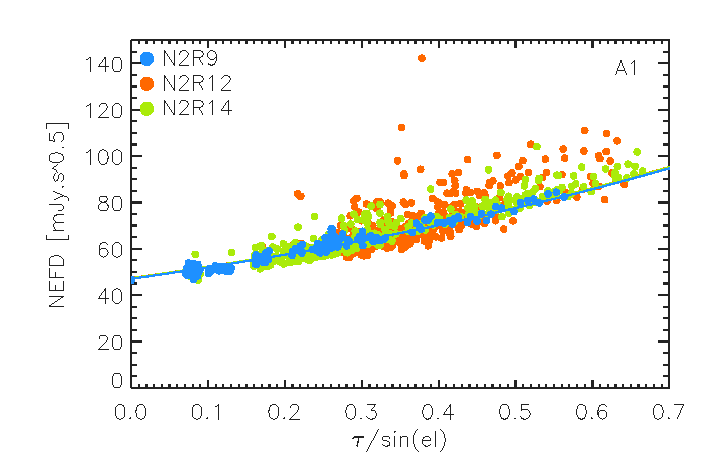
\includegraphics[clip=true,width=0.47\textwidth]{Figures/plot_nefd_vs_obstau_corrected_skydip_vfinal_a1.pdf}
%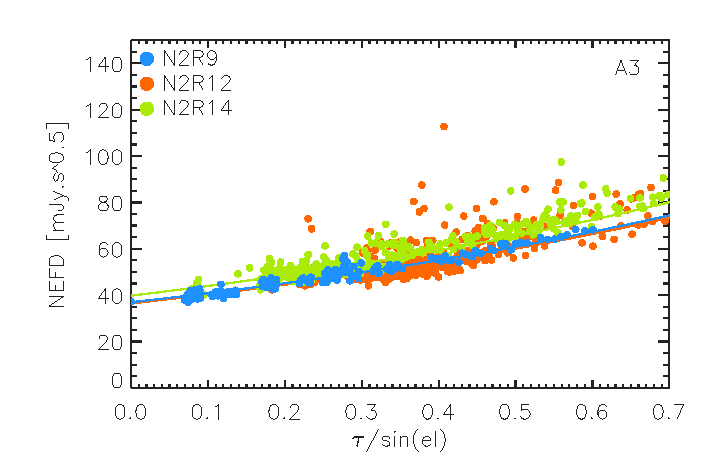
\includegraphics[clip=true,width=0.47\textwidth]{Figures/plot_nefd_vs_obstau_corrected_skydip_vfinal_a3.pdf}
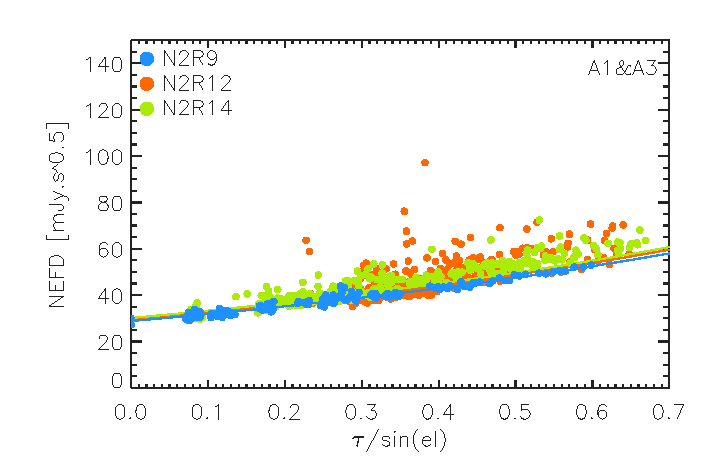
\includegraphics[clip=true,width=0.47\textwidth]{Figures/plot_nefd_vs_obstau_corrected_skydip_vfinal_1mm.pdf}
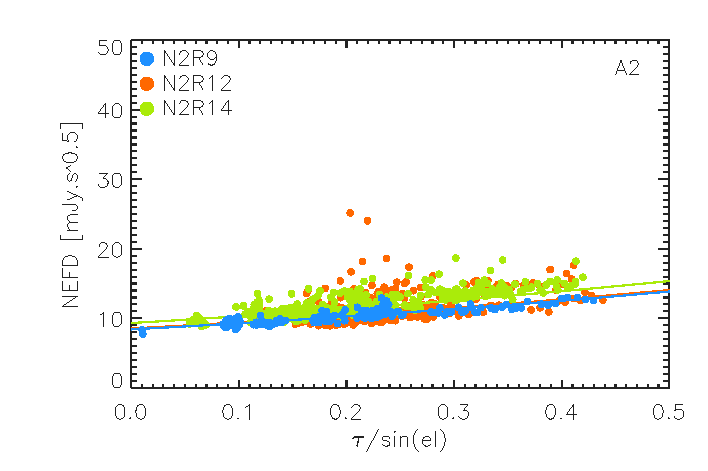
\includegraphics[clip=true,width=0.47\textwidth]{Figures/plot_nefd_vs_obstau_corrected_skydip_vfinal_a2.pdf}
\caption{Comparison of the NEFD estimates for three observation
  campaigns. The measured NEFD using the scatter method is plotted as a function of
  line-of-sight opacity ($\tau/sin(\delta)$) for the $1~\rm{mm}$ (left) and $2~\rm{mm}$ (right)
  channels. Data points are NEFD estimates in mJy.s$^{1/2}$ for N2R9 (blue), N2R12 (orange)
  and N2R14 (chartreuse). We also show in the plots the expected NEFD evolution
  with the line-of-sight opacity as solid curves using the median
  zenith opacity derived from all the scans acquired during a campaign.}
\label{fig:nefdvsbackground_below_1Jy}
\end{center}
\end{figure*}

Combining the data set of N2R9, N2R12 and N2R14 campaigns,
more than one thousand observations scans of sub-Jy sources meet the
baseline selection criteria (see Sect.~\ref{se:data_selection}),
providing us with robust NEFD estimates that are representative of
average NIKA2 performance, which are gathered in
Tab.~\ref{tab:nefd_astro}.
The top-of-atmosphere NEFD and RMS uncertainties are evaluated as the median and
the scatter of the individual NEFD corrected with
$\exp[\tau/sin(\delta)]$. These values are then extrapolated at the
reference IRAM observing conditions, which consists of $2~\rm{mm}$
of precipitable water vapor (pwv) in the atmosphere and $60$ degrees
elevation.


\subsubsection{Mapping speed}

To further estimate the mapping capabilities, we also evaluate the
mapping speed $M_{\rm{s}}$, which is defined as the sky area that is covered in one
hour of observation to a noise level of $1\,\rm{mJy}$, using
\begin{equation}
M_{\rm{s}} = \eta \, \frac{\pi}{4} d_{\rm{FoV}}^2 \, \frac{\Delta_t}{\rm{NEFD}^2},
\end{equation}
where $d_{\rm{FoV}} = 6.5'$ is the FoV diameter, $\eta$ the
fraction of valid KIDs, as given in Tab.~\ref{tab:number_of_kids} in
Sect.~\ref{se:fov_geometry} and $\Delta_t$ a time period of one hour.
The mapping speed that is extrapolated at zero opacity, and the astronomer
mapping speed that is extrapolated at the reference IRAM observing conditions are
given in Tab.~\ref{tab:nefd_astro}.   
%eta  = [0.84, 0.84, 0.84, 0.90]
%nefd0 = [47.2, 37.9, 30.1, 8.8]
%ms0   = !dpi/4.0d0*6.5d0^2*eta/nefd0^2*60.0d0^2 ;; arcmin^2/h/mJy^2
%print, ms0
%nefda = [56.6, 45.6, 36.1, 9.8]
%msa   = !dpi/4.0d0*6.5d0^2*eta/nefda^2*60.0d0^2 ;; arcmin^2/h/mJy^2
%print, msa

\begin{table}[!thbp]
  \begin{center}
    \caption[NEFD estimates on all sub-Jy sources]{Median NEFD and rms
      uncertainties in $\rm{mJy}\cdot \rm{s}^{1/2}$, as well as the derived mapping
      speed in $\rm{arcmin}^2\cdot\rm{mJy}^{-2}\cdot\rm{h}^{-1}$, evaluated
      in using the scatter method on all sub-Jy sources of runs N2R9, N2R12
      and N2R14, given at pwv=0 and 90 degrees elevation (first three rows) and extrapolated at the
      reference IRAM observing conditions (last three rows), which are defined
      as $2\,\rm{mm}$ pwv and 60 degrees elevation.}
    \label{tab:nefd_astro}
    \begin{tabular}{lrrrr}
      \hline\hline
      \noalign{\smallskip}
      <1 Jy               & A1      &   A3    &   A1\&A3 &    A2 \\
      \noalign{\smallskip}
      \hline
      \noalign{\smallskip}
      NEFD\small{(0mm, 90deg)}             & 47.2    & 37.9    &    30.1  &    8.8   \\
      RMS NEFD\small{(0mm, 90deg)}         &  3.9    &  3.5    &     2.9  &    1.1   \\
      M$_{\rm{s}}$\small{(0mm, 90deg)}      & 45      &  70     &    111   &   1388   \\
      \hline
      \noalign{\smallskip}
      NEFD\small{(2mm, 60deg)}         & 56.6    & 45.6    &    36.1  &    9.8   \\
      RMS NEFD\small{(2mm, 60deg)}     &  4.7    & 4.2     &     3.5  &    1.2   \\
      M$_{\rm{s}}$\small{(2mm, 60deg)}  &  31    & 48       &    77   &   1119   \\
      \hline
    \end{tabular}
\end{center}
\end{table}


In this section, we derive the on-sky sensitivity of the instrument
using a large amount of observation scans, including deep integration
on faint sources, to assess our result stability against the observing
conditions. We evaluate the noise equivalent flux
density, NEFD hereafter, that is the flux density
$1\,\sigma$ errors in one second of effective
on-source telescope integration time after the baseline calibration
has been performed, as described in
Sect.~\ref{se:baseline_calibration}. The first step for
the NEFD measurement is thus an accurate evaluation of the on-source
integration time, which is addressed in
Sect.~\ref{se:integration_time}. Then, for robustness test of the NEFD
estimates, we have devised several methods for estimating the NEFD. A
detailed description of our methods, as well as an application to a
faint source blind detection, will be found in
\citet{Ponthieu2019}. In Sect.~\ref{se:nefd_method}, we briefly
present the NEFD estimation methods that have been used and the data
sets that have been selected. Finally, the NEFD estimates and the
results of the robustness tests we performed are reported in
Sect.~\ref{se:nefd_results}.


\subsection{Estimation of the time of integration}
\label{se:integration_time}

Considering an observation scan of a point-like source, from which we
produce a map by projecting the calibrated TOI (see
Sect.~\ref{se:dataproc}) into pixels of size $\Delta r$, we primarily
estimate the time of integration on-source, which is the integration
time in a beam $t_{\rm{beam}}$, using
%
\begin{equation}
  t_{\rm{beam}} = \frac{<N_{\rm{hit}}>_{\rm{center}}}{f_{\rm{sam}}}\,
  \eta \frac{g^2}{\Delta_r^2},
  \label{eq:integration_time}
\end{equation}
%
where $N_{\rm{hit}}$ is the so-called hit map, that is the map of the
TOI sample count per map pixels, and $<N_{\rm{hit}}>_{\rm{center}}$
is the average of the hit map over the pixels within a FWHM radius
from the center of the map. The ratio of this quantity to the sampling
frequency $f_{\rm{sam}}$ thus corresponds to the total time of integration
spend in a map pixel of the center of the map. As all the KIDs of an
array produce a data sample at the same time, we need to correct the
total time of integration from the fraction of the KID that
contributes to a map pixel at the same time. For this purpose, first
we estimate the number of KID per map pixel as the ratio of $g^2$ to
$\Delta_r^2$, where $g$ is the distance between neighbour KIDs (see
Sect.~\ref{se:grid_distortion}). Then, we multiply
this quantity by the fraction of valid KID $\eta$ that actually
contribute to the map (see Sect.~\ref{se:avg_kidpar}). 

For cross-checks, we compare the $t_{\rm{beam}}$ estimates using an
alternative approach for evaluating the on-source integration
time based on geometrical considerations. Namely, we calculate the
fraction of the scanning time during which the point source in within
an effective FOV radius, which is defined as the FOV covered by the
valid KIDs. We find the two methods to give comparable integration
time estimates to better than $5\%$. We conclude the $t_{\rm{beam}}$
estimates to be reliable and use it for the NEFD derivation.  


\subsection{NEFD estimation methods and source selection}
\label{se:nefd_method}

We have devised three complementary methods for the
NEFD estimation, which come in two different flavours. First, we
use deep integrations on faint sources, and second we resort to 
joint analysis of multiple scans without combining them. An
extensive discussion of these methods will be given in
\citet{Ponthieu2019}. In this section, we briefly describe one method
for each of the two approaches: \\

\noindent \emph{Deep integration method:} The error on the flux
density of a point source for an integration time $t$ is
$\sigma_\phi(t) = NEFD/\sqrt{t}$. Using long-time integration
observation on a source, we can study the decrease of $\sigma_\phi$
with increasing $t$, and therefore estimate the NEFD if the
different elevation and opacity conditions of observations are
correctly accounted for.
We produce a series of maps using an inverse-variance co-addition of
more and more observation scans, and perform a photometric analysis on
each map according to Sect.~\ref{se:photometry}. Since all the scans
are not acquired in the exact same conditions of atmospheric opacity
and observing elevation, they do not contribute with the same weight
to the co-addition. To derive the top-of-atmosphere NEFD, quoted
NEFD$_0$, we account for the scan-to-scan weighting variations by fitting
the $1\sigma$ flux errors with
\begin{equation}
  \sigma(n) = \frac{NEFD_0}{\sqrt{\sum_{i=1}^{n}t_i e^{-2\tau_i/\sin\delta_i}}},
  \label{eq:sigma_tau_w8}
\end{equation}
where $t_i$, $\tau_i$ and $\delta_i$ are the integration time, the
zenith opacity and the observing elevation of the $i$-th scan of the
$n$-scan co-addition. The quantity $\sum_{i=1}^{n}t_i
e^{-2\tau_i/\sin\delta_i}$ thus consists in an
estimate of the effective integration time for the series of scans
that enter the $n$-scan co-addition. \\

\noindent \emph{Scatter method:} Performing photometry on each
individual scan, we can estimate the sensitivity on the central flux
and measure the time of integration using
Eq.~\ref{eq:integration_time}, hence derive the NEFD for this
scan. After correction of the attenuation of the atmosphere, the joint
analysis of a series of scans provides us with an estimate of the
top-of-atmosphere NEFD. \\

The selection of the source target for the NEFD derivation is
primarily based on the flux density. Indeed, noise
characterization may be biased by residuals of a strong source and the
instrument far side lobes. For the scatter method, we therefore
restrict the analysis to sources with a flux below 1\,Jy. For the deep
integration method, we further need to select a single source whose
visibility allows for long integration time. During the N2R9 campaign,
we selected \hls\, which is a
moderately faint source \citep{hls_combes}, expected to be
74.5\,mJy at 1mm and 15.7\,mJy at 2mm (M.~Bethermin, private
communication). It has been observed for about 9\,h in total over
three nights using 8x5~arcmin$^2$ OTF scans of various orientations. 

\begin{figure*}[!thbp]
  \begin{center}
    \includegraphics[trim={0.5cm, 0.5cm, 1.5cm, 1.8cm}, clip, angle=0, width=0.495\textwidth]{Figures/hls_nefd_vst.eps}
    \includegraphics[trim={0.5cm, 0, 0.2cm, 0.5cm}, clip, angle=0, width=0.485\textwidth]{Figures/hls_NEFD_vs_TauElev_all.eps}
    \caption{Comparison of NEFD estimates using two methods on
      observation of \hls. \emph{Left panel:} Evolution of the 1\,$\sigma$ flux density uncertainties as a function of the integration time; \emph{Right panel:} NEFD as a function of the measured line-of-sight opacity. The solid black line is the theoretical fit of $\rm{NEFD} = \rm{NEFD}_0$ $e^{(\tau/\sin\delta)}$ and gives the NEFD when extrapolated to $\tau/\sin\delta = 0$.}
    \label{fig:nefd_twomethods}
  \end{center}
\end{figure*}

\subsection{NEFD estimation and robustness tests}
\label{se:nefd_results}

%  comparison entre methods
First we test the stability of the NEFD estimates using the two
methods on a same data set. In Fig.~\ref{fig:nefd_twomethods}, we
present an application of the deep integration method (left panel) and
the scatter method (right panel) on
%the NEFD estimates for Array 1, 3, the combination of A1$\&$A3
%and Array 2 using
the series of \hls\ observation scans.

The left panel of Fig.~\ref{fig:nefd_twomethods} shows the flux density
uncertainties as a function of the integration time. This plot has
been obtained as discussed in Sect.~\ref{se:nefd_method}. The small
variations of the slope of the $1\sigma$ flux errors, which are
visible on the plot, correspond to variations of line-of-sight opacity
during the integration. These variations are taken into account for
evaluating the top-of-atmosphere NEFD using
Eq.~\ref{eq:sigma_tau_w8}. The NEFD estimates for Array 1, 3, the
combination of A1$\&$A3 and Array 2 using the deep  
integration method are given in the first row of
Table~\ref{tab:nefd_summary}.
 
\begin{table}[!htbp]
  \centering
  \caption[]{Stability of the NEFD estimates. Top-of-atmosphere NEFD
    in mJy.s$^{1/2}$ for the two methods described in the text and
    obtained on \hls\ and all sub-Jy sources of runs N2R9,
  N2R12, N2R14. The results given in the last row are based on more
  than a thousand scans, which distribute as 202, 481 and 430 scans of
  N2R9, N2R12 and N2R14 respectively.}
  \label{tab:nefd_summary}
  \begin{tabular}{llrrrr}
    \hline\hline
    \noalign{\smallskip}
    Data set   & Method   & A1      &   A3    &   A1\&A3 &    A2 \\
    \noalign{\smallskip}
    \hline
    \noalign{\smallskip}
    \hls &     $t^{-1/2}$  &  46.6  &    38.4  &    30.4  &   8.5  \\
    %   G2   &    $t^{-1/2}$  &  44.0  &    34.7  &    29.6  &  7.8  \\
         &     Scatter    &  45.7  &    36.3  &    28.5  &   8.2  \\
    \hline
    \noalign{\smallskip}
    N2R9     & Scatter    & 47.0 &  36.9  & 28.8  & 8.4 \\
    N2R12    &            & 47.3 &  36.4  & 30.2  & 8.5 \\
    N2R14    &            & 47.3 &  39.8  & 30.9  & 9.3 \\
    Combined &            & 47.2 &  37.9  & 30.1  & 8.8 \\
    \hline
  \end{tabular}
\end{table}

In addition, we verify that the noise integrates down as expected with
respect to the integration time. Black lines in the left panel of
Fig.~\ref{fig:nefd_twomethods} show the $1\sigma$ error fit with the
inverse of the square root of the integration time. The noise
integration is well consistent with $t^{-1/2}$.

The right panel of Fig.~\ref{fig:nefd_twomethods} show the NEFD
estimates for  Array 1, 3, the combination of A1$\&$A3 and Array 2
using the scatter method, as discussed in Sect.~\ref{se:nefd_method},
as a function of the line-of-sight opacities, $\tau/sin(\delta)$,
where $\tau$ is the zenith opacity and $\delta$ the observing
elevation. The solid lines show the best fit of the model for a
background-dominated sensitivity,
defined as NEFD = NEFD$_0$ exp${[\tau/sin(\delta)]}$. The best-fitting
NEFD$_0$ amplitude give us estimates of the
top-of-atmosphere NEFD, which are gathered in
Table~\ref{tab:nefd_summary}.

We observe systematically higher NEFD for A1 compared to
A3, which is a mainly due to the dichroic-induced 'shadow effect' that
also impacts the flat fields, as discussed in
Sect.~\ref{se:flat_field}. Furthermore, the NEFDs are well consistent
with being background dominated for each array and each observing
wavelength. 


%  comparison entre datasets
As a second robustness test, we check the stability of the NEFD for
three observation
campaigns. Figure~\ref{fig:nefdvsbackground_below_1Jy} shows the
measured NEFD using the scatter method for runs N2R9, N2R12 and
N2R14. 

\begin{figure*}[!thbp]
\begin{center}
%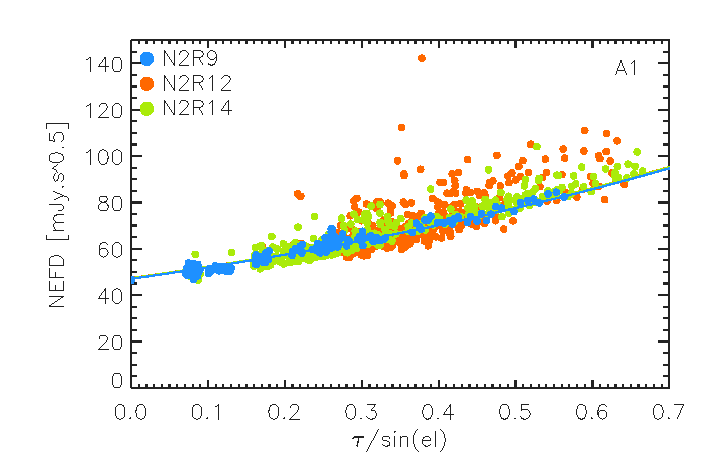
\includegraphics[clip=true,width=0.47\textwidth]{Figures/plot_nefd_vs_obstau_corrected_skydip_vfinal_a1.pdf}
%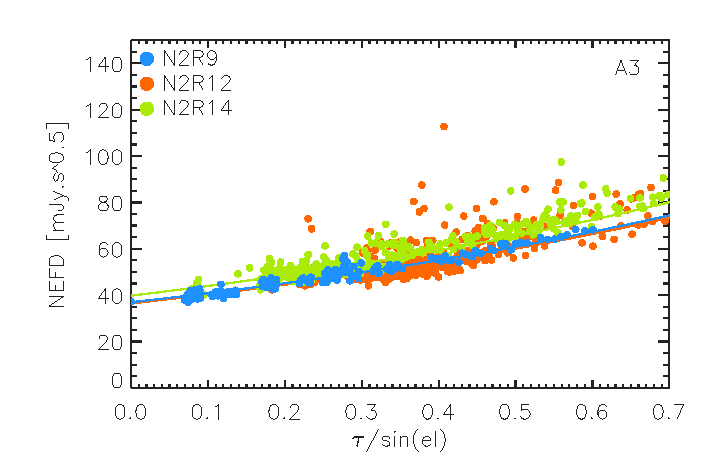
\includegraphics[clip=true,width=0.47\textwidth]{Figures/plot_nefd_vs_obstau_corrected_skydip_vfinal_a3.pdf}
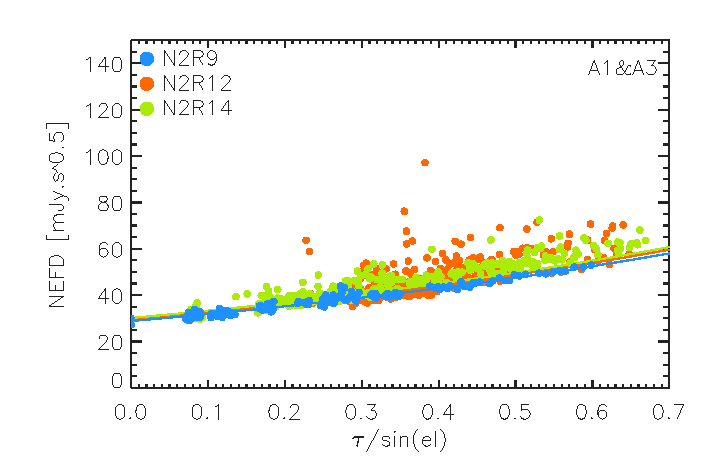
\includegraphics[clip=true,width=0.47\textwidth]{Figures/plot_nefd_vs_obstau_corrected_skydip_vfinal_1mm.pdf}
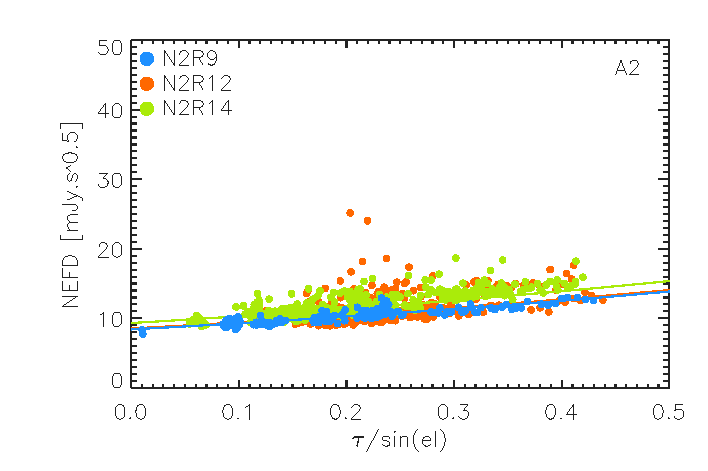
\includegraphics[clip=true,width=0.47\textwidth]{Figures/plot_nefd_vs_obstau_corrected_skydip_vfinal_a2.pdf}
\caption{Comparison of the NEFD estimates for three observation
  campaigns. The measured NEFD using the scatter method is plotted as a function of
  line-of-sight opacity ($\tau/sin(\delta)$) for the $1~\rm{mm}$ (left) and $2~\rm{mm}$ (right)
  channels. Data points are NEFD estimates in mJy.s$^{1/2}$ for N2R9 (blue), N2R12 (orange)
  and N2R14 (chartreuse). We also show in the plots the expected NEFD evolution
  with the line-of-sight opacity as solid curves using the median
  zenith opacity derived from all the scans acquired during a campaign.}
\label{fig:nefdvsbackground_below_1Jy}
\end{center}
\end{figure*}

Combining the data set of N2R9, N2R12 and N2R14 campaigns,
more than one thousand observations scans of sub-Jy sources meet the
baseline selection criteria (see Sect.~\ref{se:data_selection}),
providing us with robust NEFD estimates that are representative of
average NIKA2 performance, which are gathered in
Tab.~\ref{tab:nefd_astro}.
The top-of-atmosphere NEFD and RMS uncertainties are evaluated as the median and
the scatter of the individual NEFD corrected with
$\exp[\tau/sin(\delta)]$. These values are then extrapolated at the
reference IRAM observing conditions, which consists of $2~\rm{mm}$
of precipitable water vapor (pwv) in the atmosphere and $60$ degrees
elevation.


\subsubsection{Mapping speed}

To further estimate the mapping capabilities, we also evaluate the
mapping speed $M_{\rm{s}}$, which is defined as the sky area that is covered in one
hour of observation to a noise level of $1\,\rm{mJy}$, using
\begin{equation}
M_{\rm{s}} = \eta \, \frac{\pi}{4} d_{\rm{FoV}}^2 \, \frac{\Delta_t}{\rm{NEFD}^2},
\end{equation}
where $d_{\rm{FoV}} = 6.5'$ is the FoV diameter, $\eta$ the
fraction of valid KIDs, as given in Tab.~\ref{tab:number_of_kids} in
Sect.~\ref{se:fov_geometry} and $\Delta_t$ a time period of one hour.
The mapping speed that is extrapolated at zero opacity, and the astronomer
mapping speed that is extrapolated at the reference IRAM observing conditions are
given in Tab.~\ref{tab:nefd_astro}.   
%eta  = [0.84, 0.84, 0.84, 0.90]
%nefd0 = [47.2, 37.9, 30.1, 8.8]
%ms0   = !dpi/4.0d0*6.5d0^2*eta/nefd0^2*60.0d0^2 ;; arcmin^2/h/mJy^2
%print, ms0
%nefda = [56.6, 45.6, 36.1, 9.8]
%msa   = !dpi/4.0d0*6.5d0^2*eta/nefda^2*60.0d0^2 ;; arcmin^2/h/mJy^2
%print, msa

\begin{table}[!thbp]
  \begin{center}
    \caption[NEFD estimates on all sub-Jy sources]{Median NEFD and rms
      uncertainties in $\rm{mJy}\cdot \rm{s}^{1/2}$, as well as the derived mapping
      speed in $\rm{arcmin}^2\cdot\rm{mJy}^{-2}\cdot\rm{h}^{-1}$, evaluated
      in using the scatter method on all sub-Jy sources of runs N2R9, N2R12
      and N2R14, given at pwv=0 and 90 degrees elevation (first three rows) and extrapolated at the
      reference IRAM observing conditions (last three rows), which are defined
      as $2\,\rm{mm}$ pwv and 60 degrees elevation.}
    \label{tab:nefd_astro}
    \begin{tabular}{lrrrr}
      \hline\hline
      \noalign{\smallskip}
      <1 Jy               & A1      &   A3    &   A1\&A3 &    A2 \\
      \noalign{\smallskip}
      \hline
      \noalign{\smallskip}
      NEFD\small{(0mm, 90deg)}             & 47.2    & 37.9    &    30.1  &    8.8   \\
      RMS NEFD\small{(0mm, 90deg)}         &  3.9    &  3.5    &     2.9  &    1.1   \\
      M$_{\rm{s}}$\small{(0mm, 90deg)}      & 45      &  70     &    111   &   1388   \\
      \hline
      \noalign{\smallskip}
      NEFD\small{(2mm, 60deg)}         & 56.6    & 45.6    &    36.1  &    9.8   \\
      RMS NEFD\small{(2mm, 60deg)}     &  4.7    & 4.2     &     3.5  &    1.2   \\
      M$_{\rm{s}}$\small{(2mm, 60deg)}  &  31    & 48       &    77   &   1119   \\
      \hline
    \end{tabular}
\end{center}
\end{table}


In this section, we derive various quantities that relate to the
sensitivity of the instrument:

\begin{itemize}
\item The detector Noise Equivalent Flux Density $NEFD_{det,0}$ is the 1\,$\sigma$
  error on the flux of a point source as measured by a detector in 1~second of
  integration time.
\item The observer Noise Equivalent Flux Density $NEFD_{obs,0}$ is the 1\,$\sigma$
  error on the flux of a point source in 1~second of telescope integration time.
\item The mapping speed $M_s$ is the sky area that can be mapped at a noise
  level of 1\,mJy in one hour of telescope integration time.
\end{itemize}

Subscript $_0$ means that at this stage, we consider these definitions in
the absence of atmosphere. Corrections to account for elevation and opacity are
addressed later on. We first focus on these definitions and how to defined more
these quantities more technically in sect.\ref{se:integration_time}. Section~\ref{se:nefd_method}
presents several methods to estimate them. Results, together with robustness
tests are reported in sect.~\ref{se:nefd_results}.

\subsection{NEFD and mapping speed definitions}
\label{se:integration_time}

%% \nico{While the notion of ``observation time'' seems intuitively
%%   straightforward, it deserves a closer look when it comes to actually
%%   estimating it on data acquired with non continuous arrays of detectors. The
%%   NEFD is commonly refered to individual \emph{detectors} and must then be
%%   related to the whole \emph{instrument} to provide the observer with a mapping speed
%%   and a time estimator to plan observations.}


We distinguish the on-source \emph{detector} integration time $t_{det}$ from the
on-source \emph{observer} integration time $t_{obs}$. The former refers to the
cumulative time spent on-source by detectors, the latter to the cumulative time
spent on-source by the FOV overall as commonly considered when talking about the
``instrument being on-source''. To be even more concrete, assume that at some point during
a scan, the source is located on a region of the FOV where a few KIDs are blind: no
valid detector is actually seeing the source at this time, so $t_{det}$ is not
incremented while $t_{obs}$ is. $t_{det}$ is releveant for the estimation of detector
performances, $t_{obs}$ is relevant for astronomers when
designing scanning strategies and estimating the required observation time to
reach a given sensitivity, as we shall see in the following.

Let us consider a map of resolution $r$\,arcsec as obtained from
observations. The instantaneous $A$ covered by the FOV reads

\begin{equation}
A = \pi d_{FOV}^2/4 = N_{pix}r^2 = N_k g^2,
\end{equation}

where $d_{FOV}$ is the FOV diameter, $N_{pix}$ the number of map pixels inside
this area, $N_k$ the number of designed KIDs of an array
(Table~\ref{tab:number_of_kids}) and $g$ the distance between two adjacent
KIDs. Assume that the instrument remains fix on the sky for an observer time
$t_{obs}$, the total number of samples acquired during this time and spread on
the entire FOV is $\eta N_k t_{obs} f_{\rm{sam}}$ where $\eta$ is the fraction
of valid KIDs (tab.~\ref{tab:number_of_kids}). This leads to an average
observation time per map pixel

\begin{equation}
\langle t_{pix}\rangle = \langle N_{\rm{hit}}\rangle f_{\rm{sam}} = \eta N_k
t_{obs} f_{\rm{sam}}/N_{pix},
\end{equation}

and thus to

\begin{equation}
  t_{obs} = \frac{1}{\eta}\frac{\langle N_{\rm{hit}}\rangle_{\rm{center}}}{f_{\rm{sam}}}\,
  \frac{g^2}{r^2}.
\label{eq:t_obs}
\end{equation}

where we have added the subscript \emph{center} to specify that in order to
estimate $t_{obs}$ from the map, we take the number of hits per pixel at the map
center. In practice, we take the average of this number in a disk of radius
1\,FWHM to be immune to shot noise statistics in map pixels. The on-source
detector integration time then reads

\begin{equation}
t_{det} = \eta t_{obs}
\label{eq:t_det}
\end{equation}

If all KIDs are valid, $\eta$ equals 1 and the two integration times match, the
lower $\eta$, the lower the time actually spent on-source by detectors for the
same $t_{obs}$. An alternate way to derive $t_{obs}$ is to measure, during
observations, the amount of time when the source is at less than $d_{FOV}/2$
from the FOV center. This method gives values of $t_{obs}$ that agree with
eq.~(\ref{eq:t_obs}) to better than 5\%. In this work, we consider $t_{obs}$ as
given by eq.~(\ref{eq:t_obs}) because it is derived from the final map and can
therefore be generalized to any other place on the map than its center.

From these definitions and for the same $\sigma$ error on the measured flux of
the point source, we can now derive the corresponding NEFDs:

\begin{eqnarray}
NEFD_{det,0} & = & \sigma \sqrt{t_{det}} \label{eq:nefd_det},\\
NEFD_{obs,0} & = & \sigma \sqrt{t_{obs}} \label{eq:nefd_obs}.
\end{eqnarray}

Considering the surface covered by the FOV, we define the \emph{mapping speed}
as the surface that can be mapped at a given sensitivity in a certain
observation time and which reads

\begin{equation}
M_s = \eta \, \frac{\pi}{4} d_{\rm{FoV}}^2 \, \frac{1}{(NEFD_{det,0})^2}
\label{eq:mapping_speed}
\end{equation}

\subsection{NEFD estimation methods and scan selection}
\label{se:nefd_method}

We have devised three complementary methods for the
NEFD estimation, which come in two different flavours. First, we
use deep integrations on faint sources, and second we resort to 
joint analysis of multiple scans without combining them.\\
%% An
%% extensive discussion of these methods will be given in
%% \citet{Ponthieu2019}. In this section, we briefly describe one method
%% for each of the two approaches: \\

\noindent \emph{Deep integration method:} The error on the flux density of a
point source for an integration time $t_{det}$ \nico{at an elevation $el$ and
  with opacity $\tau$ is $\sigma_\phi(t) = NEFD_{det,0}\,e^{\tau/\sin
    el}/\sqrt{t_{det}}$}. Using long-time integration observation on a source,
we can study the decrease of $\sigma_\phi$ with integration time, and
therefore estimate the NEFD if the different elevation and opacity conditions of
observations are correctly accounted for.  We produce a series of maps using an
inverse-variance co-addition of more and more observation scans, and perform a
photometric analysis on each map according to Sect.~\ref{se:photometry}. Since
all the scans are not acquired in the exact same conditions of atmospheric
opacity and observing elevation, they do not contribute with the same weight to
the co-addition. \nico{In such case, eq.~(\ref{eq:nefd_det}) generalizes to}

\begin{equation}
  \sigma(n) = \frac{NEFD_{det,0}}{\sqrt{\sum_{i=1}^{n}t_i e^{-2\tau_i/\sin\elev_i}}},
  \label{eq:sigma_tau_w8}
\end{equation}
where $t_i$, $\tau_i$ and $\elev_i$ are the integration time, the zenith
opacity and the observing elevation of the $i$-th scan of the $n$-scan
co-addition. \nico{Fitting $\sigma(n)$ vs the corresponding effective
  integration time $\sum_{i=1}^{n}t_i e^{-2\tau_i/\sin\elev_i}$ provides an
  estimate of $NEFD_{det,0}$. This method requires long integration on a same
  object. During the N2R9 run, we selected \hls\, a moderately faint source
  \citep{2012A&A...538L...4C}, expected to be 74.5\,mJy at 1mm and 15.7\,mJy at 2mm
  (M.~Bethermin, private communication). It has been observed for about 9\,h in
  total over three nights using 8x5~arcmin$^2$ OTF scans of various
  orientations.}\\

\noindent \emph{Scatter method:} Performing photometry on each individual scan,
we can estimate the sensitivity on the central flux and measure the time of
integration using Eq.~\ref{eq:t_det}, hence derive the NEFD per scan
scan. After correction of the attenuation of the atmosphere, the joint analysis
of a series of scans, \nico{even of different point sources,} provides us with
an estimate of the top-of-atmosphere NEFD. The selection of the source target
for the NEFD derivation is primarily based on the flux density. Indeed, noise
characterization may be biased by residuals of a strong source and the
instrument far side lobes. For this method, we therefore restrict the
analysis to sources with a flux below 1\,Jy.

\begin{figure*}[!thbp]
  \begin{center}
    \includegraphics[trim={0.5cm, 0.5cm, 1.5cm, 1.8cm}, clip, angle=0, width=0.495\textwidth]{Figures/hls_nefd_vst.eps}
    \includegraphics[trim={0.5cm, 0, 0.2cm, 0.5cm}, clip, angle=0, width=0.485\textwidth]{Figures/hls_NEFD_vs_TauElev_all.eps}
    \caption{Comparison of NEFD estimates using two methods on
      observation of \hls. \emph{Left panel:} Evolution of the 1\,$\sigma$ flux density uncertainties as a function of the integration time; \emph{Right panel:} NEFD as a function of the measured line-of-sight opacity. The solid black line is the theoretical fit of $\rm{NEFD} = \rm{NEFD}_0$ $e^{(\tau/\sin\elev)}$ and gives the NEFD when extrapolated to $\tau/\sin\elev = 0$.}
    \label{fig:nefd_twomethods}
  \end{center}
\end{figure*}

\subsection{NEFD estimation and robustness tests}
\label{se:nefd_results}

%  comparison entre methods
First we test the stability of the NEFD estimates using the two
methods on a same data set. In Fig.~\ref{fig:nefd_twomethods}, we
present an application of the deep integration method (left panel) and
the scatter method (right panel) on
%the NEFD estimates for Array 1, 3, the combination of A1$\&$A3
%and Array 2 using
the series of \hls\ observation scans.

The left panel of Fig.~\ref{fig:nefd_twomethods} shows the flux density
uncertainties as a function of the integration time. This plot has
been obtained as discussed in Sect.~\ref{se:nefd_method}. The small
variations of the slope of the $1\sigma$ flux errors, which are
visible on the plot, correspond to variations of line-of-sight opacity
during the integration. These variations are taken into account for
evaluating the top-of-atmosphere NEFD using
Eq.~\ref{eq:sigma_tau_w8}. The NEFD estimates for Array 1, 3, the
combination of A1$\&$A3 and Array 2 using the deep  
integration method are given in the first row of
Table~\ref{tab:nefd_summary}.
 
\begin{table}[!htbp]
  \centering
  \caption[]{Stability of the NEFD estimates. Top-of-atmosphere NEFD
    in mJy.s$^{1/2}$ for the two methods described in the text and
    obtained on \hls\ and all sub-Jy sources of runs N2R9,
  N2R12, N2R14. The results given in the last row are based on more
  than a thousand scans, which distribute as 202, 481 and 430 scans of
  N2R9, N2R12 and N2R14 respectively.}
  \label{tab:nefd_summary}
  \begin{tabular}{llrrrr}
    \hline\hline
    \noalign{\smallskip}
    Data set   & Method   & A1      &   A3    &   A1\&A3 &    A2 \\
    \noalign{\smallskip}
    \hline
    \noalign{\smallskip}
    \hls &     $t^{-1/2}$  &  46.6  &    38.4  &    30.4  &   8.5  \\
    %   G2   &    $t^{-1/2}$  &  44.0  &    34.7  &    29.6  &  7.8  \\
         &     Scatter    &  45.7  &    36.3  &    28.5  &   8.2  \\
    \hline
    \noalign{\smallskip}
    N2R9     & Scatter    & 47.0 &  36.9  & 28.8  & 8.4 \\
    N2R12    &            & 47.3 &  36.4  & 30.2  & 8.5 \\
    N2R14    &            & 47.3 &  39.8  & 30.9  & 9.3 \\
    Combined &            & 47.2 &  37.9  & 30.1  & 8.8 \\
    \hline
  \end{tabular}
\end{table}

In addition, we verify that the noise integrates down as expected with
respect to the integration time. Black lines in the left panel of
Fig.~\ref{fig:nefd_twomethods} show the $1\sigma$ error fit with the
inverse of the square root of the integration time. The noise
integration is well consistent with $t^{-1/2}$.

The right panel of Fig.~\ref{fig:nefd_twomethods} show the NEFD
estimates for  Array 1, 3, the combination of A1$\&$A3 and Array 2
using the scatter method, as discussed in Sect.~\ref{se:nefd_method},
as a function of the line-of-sight opacities, $\tau/sin(\elev)$,
where $\tau$ is the zenith opacity and $\elev$ the observing
elevation. The solid lines show the best fit of the model for a
background-dominated sensitivity,
defined as NEFD = NEFD$_0$ exp${[\tau/sin(\elev)]}$. The best-fitting
NEFD$_0$ amplitude give us estimates of the
top-of-atmosphere NEFD, which are gathered in
Table~\ref{tab:nefd_summary}.

We observe systematically higher NEFD for A1 compared to
A3, which is a mainly due to the dichroic-induced 'shadow effect' that
also impacts the flat fields, as discussed in
Sect.~\ref{se:flat_field}. Furthermore, the NEFDs are well consistent
with being background dominated for each array and each observing
wavelength. 

%  comparison entre datasets
As a second robustness test, we check the stability of the NEFD for
three observation campaigns. Figure~\ref{fig:nefdvsbackground_below_1Jy} shows the
measured NEFD using the scatter method (see Sect.~\ref{se:nefd_method}) for the
sub-Jansky sources acquired at the N2R9, N2R12 and N2R14
campaigns. The NEFD estimates for the
three campaigns are in agreement within uncertainties for the whole
range of line-of-sight opacities that have been tested.
The solid lines show the expected dependance with
exp${[\tau/sin(\elev)]}$ for a background-limited sensitivity
model. Since the measured NEFD are not Gaussian distributed, we
derive the top-of-atmosphere NEFD as the median of the measured NEFD
per scans after correction of the atmospheric attenuation, which provides us
with a more robust estimate compared to a fit. The NEFD$_0$ estimates
are given in Table~\ref{tab:nefd_summary}.

Combining the data set of N2R9, N2R12 and N2R14 campaigns,
more than one thousand observations scans of sub-Jy sources meet the
baseline selection criteria (see Sect.~\ref{se:data_selection}),
providing us with robust NEFD estimates that are representative of
average NIKA2 performance, which are gathered in
Table~\ref{tab:nefd_astro}.
The RMS uncertainties are evaluated as the rms scatter of the
individual NEFD estimates after correction with
$\exp[\tau/sin(\elev)]$. These values are then extrapolated at the
reference IRAM observing conditions, which consists of $2~\rm{mm}$
of precipitable water vapor (pwv) in the atmosphere and $60$ degrees
elevation.  

\begin{figure*}[!thbp]
\begin{center}
%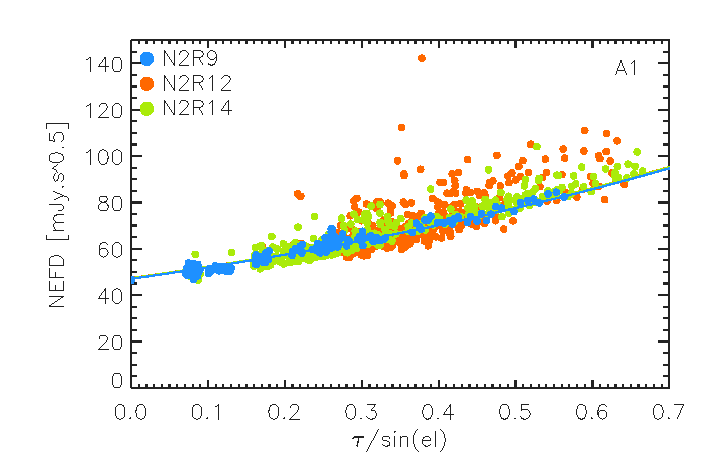
\includegraphics[clip=true,width=0.47\textwidth]{Figures/plot_nefd_vs_obstau_corrected_skydip_vfinal_a1.pdf}
%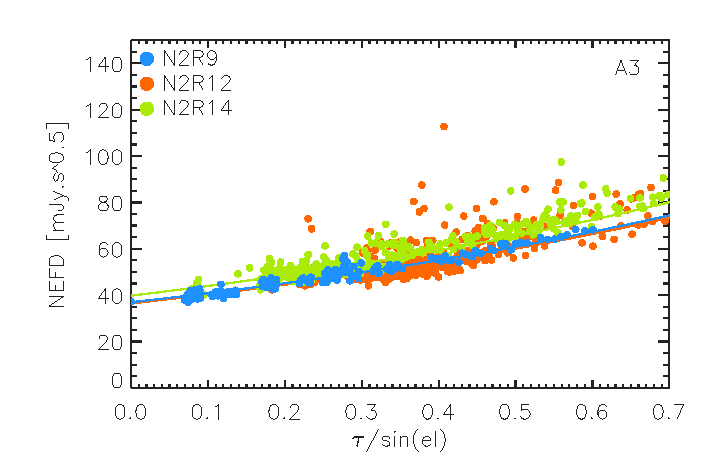
\includegraphics[clip=true,width=0.47\textwidth]{Figures/plot_nefd_vs_obstau_corrected_skydip_vfinal_a3.pdf}
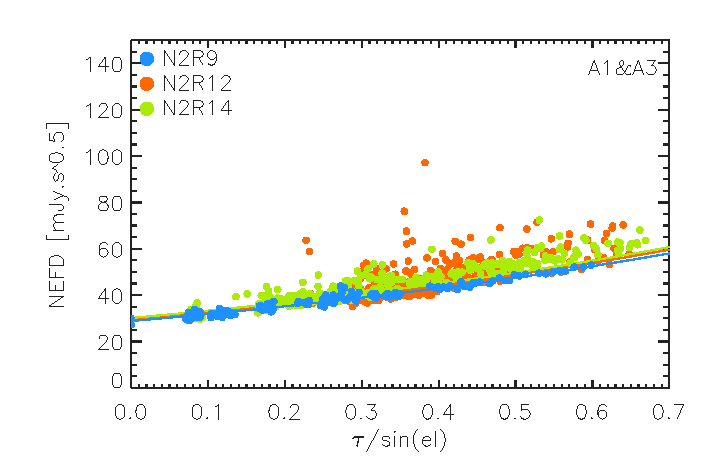
\includegraphics[clip=true,width=0.47\textwidth]{Figures/plot_nefd_vs_obstau_corrected_skydip_vfinal_1mm.pdf}
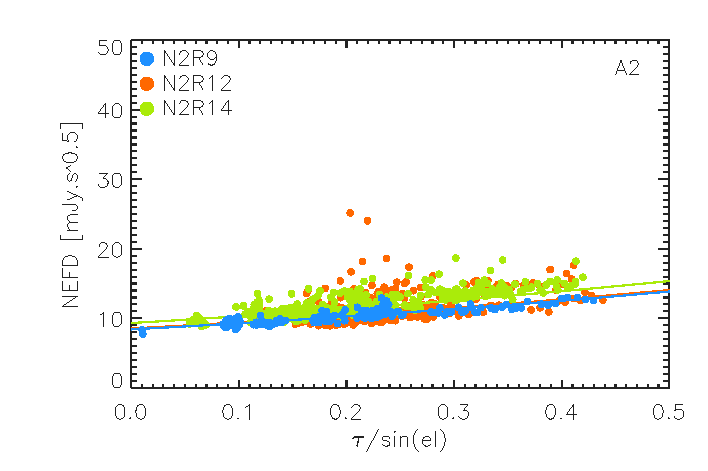
\includegraphics[clip=true,width=0.47\textwidth]{Figures/plot_nefd_vs_obstau_corrected_skydip_vfinal_a2.pdf}
\caption{Comparison of the NEFD estimates for three observation
  campaigns. The measured NEFD using the scatter method is plotted as a function of
  line-of-sight opacity ($\tau/sin(\elev)$) for the $1~\rm{mm}$ (left) and $2~\rm{mm}$ (right)
  channels. Data points are NEFD estimates in mJy.s$^{1/2}$ for N2R9 (blue), N2R12 (orange)
  and N2R14 (chartreuse). We also show in the plots the expected NEFD evolution
  with the line-of-sight opacity as solid curves using the median
  zenith opacity derived from all the scans acquired during a campaign.}
\label{fig:nefdvsbackground_below_1Jy}
\end{center}
\end{figure*}


%% \subsubsection{Mapping speed}
%% 
%% To further estimate the mapping capabilities, we also evaluate the
%% mapping speed $M_{\rm{s}}$, which is defined as the sky area
%% $\mathcal{A}_{\rm{scan}}$ that can
%% be mapped at a noise level $\Delta_\sigma$ of $1\,\rm{mJy}$ in an
%% integration time $\Delta_t$ of one hour, using
%% \begin{equation}
%% M_{\rm{s}} = \frac{\mathcal{A}_{\rm{scan}}}{\Delta_\sigma\Delta_t} = \eta \, \frac{\pi}{4} d_{\rm{FoV}}^2 \, \frac{1}{\rm{NEFD}^2},
%% \end{equation}
%% where $d_{\rm{FoV}} = 6.5'$ is the FoV diameter, $\eta$ the
%% fraction of valid KIDs, as given in Tab.~\ref{tab:number_of_kids} in
%% Sect.~\ref{se:fov_geometry}. This indicates the speed at which the sky
%% can be surveyed at a flux density rms error level of $1\,\rm{mJy}$.
%% The top-of-atmosphere mapping speed, which is extrapolated at zero opacity, and the astronomer
%% mapping speed, which is extrapolated at the reference IRAM observing conditions, are
%% given in Table~\ref{tab:nefd_astro}.   
%% %eta  = [0.84, 0.84, 0.84, 0.90]
%% %nefd0 = [47.2, 37.9, 30.1, 8.8]
%% %ms0   = !dpi/4.0d0*6.5d0^2*eta/nefd0^2*60.0d0^2 ;; arcmin^2/h/mJy^2
%% %print, ms0
%% %nefda = [56.6, 45.6, 36.1, 9.8]
%% %msa   = !dpi/4.0d0*6.5d0^2*eta/nefda^2*60.0d0^2 ;; arcmin^2/h/mJy^2
%% %print, msa
%% % sig_nefd0 = [3.9, 3.5, 2.9, 1.1]
%% % sig_ms0   = !dpi/4.0d0*6.5d0^2*eta/nefd0^3*60.0d0^2*sig_nefd0

\begin{table}[!thbp]
  \begin{center}
    \caption[NEFD estimates on all sub-Jy sources]{Median NEFD and rms
      uncertainties in $\rm{mJy}\cdot \rm{s}^{1/2}$, as well as the derived mapping
      speed and mapping speed uncertainties in $\rm{arcmin}^2\cdot\rm{mJy}^{-2}\cdot\rm{h}^{-1}$, evaluated
      in using the scatter method on all sub-Jy sources of runs N2R9, N2R12
      and N2R14, given at pwv=0 and 90 degrees elevation (first three rows) and extrapolated at the
      reference IRAM observing conditions (last three rows), which are defined
      as $2\,\rm{mm}$ pwv and 60 degrees elevation.}
    \label{tab:nefd_astro}
    \begin{tabular}{lrrrr}
      \hline\hline
      \noalign{\smallskip}
      <1 Jy               & A1      &   A3    &   A1\&A3 &    A2 \\
      \noalign{\smallskip}
      \hline
      \noalign{\smallskip}
      NEFD\small{(0mm, 90deg)}             & 47.2    & 37.9    &    30.1  &    8.8   \\
      RMS NEFD\small{(0mm, 90deg)}         &  3.9    &  3.5    &     2.9  &    1.1   \\
      M$_{\rm{s}}$\small{(0mm, 90deg)}      & 45      &  70     &    111   &   1388   \\
      RMS M$_{\rm{s}}$\small{(0mm, 90deg)}  &  4      &   6     &     11   &    174   \\
      \hline
      \noalign{\smallskip}
      NEFD\small{(2mm, 60deg)}             & 56.6    & 45.6    &    36.1  &    9.8   \\
      RMS NEFD\small{(2mm, 60deg)}         &  4.7    & 4.2     &     3.5  &    1.2   \\
      M$_{\rm{s}}$\small{(2mm, 60deg)}      &  31    & 48       &    77   &   1119   \\
      RMS M$_{\rm{s}}$\small{(2mm, 60deg)}  &   3    &  4       &     7     &  137   \\
      \hline
    \end{tabular}
\end{center}
\end{table}
